\documentclass{article}
\usepackage[top=1in, bottom=1in, left=1.5in, right=1.5in]{geometry}
\usepackage{graphicx}
\usepackage{hhline}
\usepackage{listings}
\usepackage{url}

\lstset{basicstyle=\ttfamily \scriptsize,
  basicstyle=\ttfamily,
   columns=fullflexible,
   breaklines=true,
   numbers=left,
   numberstyle=\scriptsize,
   stepnumber=1,
   mathescape=false,
   tabsize=2,
   showstringspaces=false
}

\usepackage{newfloat}
\DeclareFloatingEnvironment[fileext=lol, name=Listing]{listing}

\begin{document}
\title{SE101---Lab Introduction}
\author{Rollen D'Souza, Patrick Lam, Mahesh Tripunitara}
\date{Fall 2016\\Last Updated \today}
\maketitle

This document explains how to setup and use the Tiva C Series (TM4C123G) board you have been provided using the Energia Integrated Development Environment (IDE)~\cite{tivaBoard}. Consider this an introduction to help familiarize you with the microcontroller and programming environment, not a comprehensive guide.  For more information about the board, see the documents referenced by this guide as well as those cited on Learn.

\section*{Tiva C Series---TM4C123G}
The Tiva C Series microcontroller board is a versatile, yet reasonably powerful, board designed and produced by Texas Instruments.  Your specific board is generally used to evaluate the Tiva C Series Architecture, which they describe as:
\begin{quotation}
Targeting performance and flexibility, the Tiva C Series architecture offers a 80 MHz Cortex-M with FPU, a variety of integrated memories and multiple programmable GPIO. Tiva C Series devices offer consumers compelling cost-effective solutions by integrating application-specific peripherals and providing a comprehensive library of software tools which minimize board costs and design-cycle time. Offering quicker time-to-market and cost savings, the Tiva C Series microcontrollers are the leading choice in high-performance 32-bit applications.~\cite{tivaArch}
\end{quotation}

\section*{Energia}
Energia is the Integrated Development Environment (IDE) you will use to compile and deploy code onto your microcontroller board~\cite{energia}.  If you are not using the lab computers, you can download Energia from \url{http://energia.nu}.  Energia is already pre-installed on the lab computers and can be started by:
\begin{enumerate}
	\item {[Windows] Click the Start Button}
	\item Click on Run
	\item Paste: \texttt{Q:\textbackslash eng\textbackslash ece\textbackslash energia-0101E0016}
	\item Run
\end{enumerate}
\begin{figure}[ht]
\centering
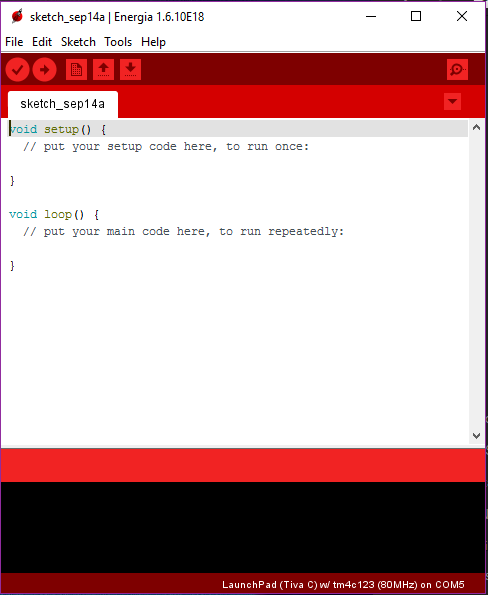
\includegraphics[width=2.5in]{Images/Energia.PNG}
\caption{Energia on startup.}
\label{fig:energiaStart}
\end{figure}
Once Energia starts, you will see something that looks like Figure \ref{fig:energiaStart}. For now, ignore the code generated by Energia. Instead, first ensure that your computer can communicate with your board. To do this, check to see that Energia is looking for the correct board model by:
\begin{enumerate}
	\item Select \emph{Tools}
	\item Select \emph{Board}
	\item Now scroll to find and select: LaunchPad (Tiva C) w/tmc4c123g (80Mhz)
\end{enumerate}
Then you need to verify that Energia communicates over the correct port. To do this:
\begin{enumerate}
	\item Select \emph{Tools}
	\item Select \emph{Serial Port}
	\item You should find two COM options. Make sure to select COM3 (a checkmark appears besides the selected option). \emph{Note that this choice is only guaranteed to work on lab computers. The correct COM port may be different on your personal machine.}
\end{enumerate}
With that, you are all set to communicate with the board! To test that everything works, press the red right arrow button (second button from the left) and read the black console at the bottom.  After a slew of messages, you should see ``Success!'' printed.

\section*{Your First Tiva Program}
You may have noticed that Energia generates a bit of code for you in the editor, namely the two functions \texttt{setup} and \texttt{loop}.  The \texttt{setup} function is executed exactly once, immediately after the code is loaded onto the board.  Normally, this function is used to initialize variables and configure pins to be inputs or outputs.  The \texttt{loop} function is where most of your code will reside.  It is executed repeatedly until you turn off the board or load a new program.

Let us begin coding! Listing~\ref{lst:blinkCode} shows an example program that flashes a light emitting diode (LED). By the way, we absolutely expect your code to have fewer comments than that in Listing~\ref{lst:blinkCode}; it is excessive and for explanatory purposes only. Use good variable names and explain anything that's unexpected (or better yet, rewrite that code.)

\begin{listing}[ht]
\lstset{basicstyle=\small, numbers=left, numbersep=3pt}
\begin{lstlisting}
// Define LED to refer to the RED LED.
#define LED RED_LED

void setup() {
	// Configure the LED pin to be an output.
	pinMode(LED, OUTPUT);
}

void loop() {
	// Raise the voltage across the LED pin.
	digitalWrite(LED, HIGH);

	// Wait for 5 seconds (LED stays on).
	delay(5000);

	// Drop the voltage across the LED pin.
	digitalWrite(LED, LOW);

	// Wait another 5 seconds (LED stays off).
	delay(5000);
}
\end{lstlisting}
\caption{Flashing the Red LED.}
\label{lst:blinkCode}
\end{listing}

This program will turn the red LED on and then off, alternating every 5 seconds.  The sequence will repeat forever.  Let us inspect the code closely:
\begin{itemize}
	\item Line 2: \texttt{\#define} allows us to to give another name for some expression. In this case, we have redefined \texttt{LED} so that it will mean \texttt{RED\_LED}. The compiler implements this by simply replacing all instances of \texttt{LED} with \texttt{RED\_LED}. You might be wondering: where is \texttt{RED\_LED} defined? It can be found in the hardware header for this board. You might also be wondering: why are we doing this? Well, if we wanted to refer to a hypothetical \texttt{GREEN\_LED} instead of \texttt{RED\_LED}, a single change to the \texttt{\#define} would suffice.

	\item Line 6: \texttt{pinMode(LED, OUTPUT)} configures the board to use the LED pin as an output pin.  You \emph{must} do this to permit modification of the LED state by changing voltage between \texttt{HIGH} and \texttt{LOW}.  You are only required to do this once for your program, before modifying LED state, and this is why it is placed within the \texttt{setup} function.

	\item Line 11: \texttt{digitalWrite(LED, HIGH)} raises the voltage across the pin connected to the LED.  The function takes two parameters, a pin and the new state: \texttt{HIGH} or \texttt{LOW}.  Although in this circumstance \texttt{HIGH} illuminates the LED, not all pins behave in this intuitive manner!  Read the documentation of the board to determine which state results in which behaviour.

	\item Line 14 - \texttt{delay(5000)} waits for 5 seconds. \texttt{delay}'s first parameter is the amount of milliseconds to wait.

\end{itemize}

After entering your code, you need to \emph{compile} and \emph{upload} your code to the board.  To compile your code, simply click the check mark icon (first button from the top left).  You can check for successful compilation in the black console at the bottom.  Once you have compiled your code, you can upload the code using the right arrow button beside the compile button.  \emph{You must compile and then upload your code everytime you modify it. Any experienced person will have been bitten by the ``running the wrong code'' problem more than once.}

Now you are ready to create more complicated programs.  Obviously you may need to use more devices than just the \texttt{RED\_LED}!  Pin defines can be found in the Energia guide on Launchpad TM4C123GXL~\cite{energiaLaunchpadGuide}.

Aside from that guide, Energia has a wealth of examples that you can learn from, including a demo of how the LCD works on the Orbit Booster Pack.  Demos can be found under \emph{File/Examples} in the Energia main menu.  The LCD example is found under the \emph{OrbitBoosterPack} sublevel.


\begin{flushleft}
\begin{thebibliography}{3}

\bibitem{tivaBoard}
	Texas Instruments.
	(2014).
	\emph{ARM\textregistered Cortex\textregistered-M4F Based MCU TM4C123G Launchpad\texttrademark Evaluation Kit} [Online].
	Available: http://www.ti.com/tool/ek-tm4c123gxl

\bibitem{tivaArch}
	Texas Instruments.
	(2014).
	\emph{Tiva\texttrademark TM4C123GH6PM Microcontroller Data Sheet} (Rev. E) [pdf].
	Available: http://www.ti.com/lit/pdf/spms376

\bibitem{energia}
	Energia.
	(2016).
	\emph{Energia} [Online].
	Available: http://energia.nu/

\bibitem{energiaLaunchpadGuide}
	Energia.
	(2016).
	\emph{Guide\_TM4C123Launchpad | Energia} [Online].
	Available: http://energia.nu/pin-maps/guide\_tm4c123launchpad/


\end{thebibliography}
\end{flushleft}

\end{document}
